% !TEX program = pdflatex
%
% DRAFT MANUSCRIPT — machine-prepared summary of the qpsim Figure-6
% reproduction campaign (2026-07-30). Every number in this draft is
% traceable to a committed, hash-bound evidence artifact in the qpsim
% repository (validation/paper_data/fischer_2023/fig6/). All physics
% claims, the author list, the venue, and the framing REQUIRE HUMAN
% PHYSICIST REVIEW before any submission. Q0 full-curve figures are
% pending the diagnostic sweep and are marked TODO.
%
\documentclass[reprint,amsmath,amssymb,aps,prapplied,nofootinbib]{revtex4-2}

\usepackage{graphicx}
\usepackage{booktabs}
\usepackage{hyperref}
\usepackage{xcolor}

\newcommand{\todo}[1]{\textcolor{red}{[TODO: #1]}}
\newcommand{\qpsim}{\textsc{qpsim}}
\newcommand{\ueV}{\,\mu\mathrm{eV}}

\begin{document}

\title{Bit-level reproduction of a driven quasiparticle-kinetics benchmark
and the sampling-convention sensitivity of gap-suppression figures}

\author{\todo{author list and affiliations}}

\date{\today\ --- DRAFT, not for distribution}

\begin{abstract}
Numerical figures in nonequilibrium superconductivity are routinely used
as benchmarks for new kinetic codes, yet the discretization conventions
behind them are rarely reported at the level a reproduction requires.  We
introduce a component-substitution validation method --- a
\emph{reproduction ladder} --- and apply it to Figure~6 of Fischer and
Catelani [Phys.\ Rev.\ Applied \textbf{XX} (2023)], which shows the
suppression of the superconducting gap under a sub-gap photon drive.
Starting from the authors' own program, we first reproduce their plotted
ordinate exactly (to the last floating-point bit) with an independent
numerical port, then replace one scientific component at a time ---
observable, parameters, energy grid, photon operator, electron--phonon
operators, phonon balance, and finally the nonlinear solver --- with the
corresponding public component of our open kinetic solver \qpsim{},
comparing every collision channel on identical frozen states before any
re-solve.  All collision physics agrees to within a few parts in
$10^{15}$.  The entire historical discrepancy between the codes ---
$33\text{--}39\%$ on the rising branch of the published figure --- is
attributed to three labeled numerical choices, dominated by a half-bin
difference in where the occupation function is sampled on the energy
grid: the same solved state reads $0.1454$ under the authors' left-edge
convention and $0.0505$ under the cell-center convention at the anchor
point, versus the published $0.1209$.  Two smaller policy differences ---
the one-bin labeling of recombination-phonon frequencies and an analytic
(Kaplan) treatment of the near-threshold pair-breaking quadrature that
the original midpoint sum overestimates by up to $27\%$ per bin --- are
isolated with dedicated controls.  Grid refinement to $\mathrm{d}E = 0.125\ueV$ shows the center-carrier
reading stable within $\pm 3\%$ while the left-edge reading falls
monotonically by $23\%$, with the inter-convention gap decaying more
slowly than $\sqrt{\mathrm{d}E}$ --- the published observable carries a
discretization offset comparable to the inter-code discrepancy itself,
and is not continuum-converged under either reading at any practical
resolution.  We argue that figures constructed
from ratios of nearly equal gap shifts amplify such sampling offsets by
more than an order of magnitude, and recommend that published kinetic
benchmarks state their sampling convention and demonstrate grid
convergence of the plotted observable.
\end{abstract}

\maketitle

\section{Introduction}

Nonequilibrium quasiparticle (QP) kinetics in superconducting devices ---
readout-induced QP generation, phonon trapping, gap suppression under
microwave drive --- is increasingly modeled with dedicated kinetic
solvers.  When a new solver is introduced, the community reasonably asks
that it reproduce established results.  This paper is about what
``reproduce'' should mean, and about a specific, quantitatively large
pitfall we found when we held ourselves to a strict standard.

\qpsim{} is an open kinetic solver for driven superconducting QP and
phonon distributions \todo{one-paragraph software description: energy
grid, collision operators, diffusion tier, junction layer; cite
repository/release}.  As part of its validation we targeted Figure~6 of
Fischer and Catelani~\cite{fischer2023} (henceforth F\&C), which plots
the normalized gap suppression of a superconductor driven by a sub-gap
photon mode of energy $\omega_0 = 20\ueV$ against an effective drive
temperature $T^*/\Delta$, for bath temperatures $T_B \in \{0.10, 0.15,
0.20\}\,$K.  Our initial comparison showed \qpsim{} lower than the
published solid curves by $33\text{--}39\%$ on the rising branch --- far
outside any acceptable tolerance, and, importantly, a discrepancy whose
cause could not be localized by staring at final curves.

The authors kindly provided the program used to produce the figure
\todo{confirm acknowledgment wording with F\&C}.  This enabled a
validation design in which the question ``why do the codes disagree?''
is answered constructively: by transforming one program into the other,
one scientific component at a time, with machine-checked evidence at
every step.

Three results came out of this campaign.
\emph{First}, a bit-level reproduction: an independent numerical port
reproduces the authors' plotted ordinate at an anchored point exactly,
and \qpsim{}'s public observable, parameters, grid, photon operator,
electron--phonon operators, and phonon balance each reproduce the
corresponding author computation to within a few parts in $10^{15}$ on
identical states.  We additionally replayed the authors' program in
full: all 300 sweep points converge under their Newton policy in 2--4
iterations, the anchored ordinate reproduces to the last bit, and the
replayed curves agree with an independent digitization of the
published raster within $0.12\times$ its declared uncertainty ---
so the exact published curves, not raster estimates, serve as the
comparison ground truth below.  \emph{Second}, an attribution: the entire historical
discrepancy reduces to three labeled numerical choices, none of which is
a defect in the collision physics of either code.  \emph{Third}, a
warning of general interest: the plotted observable is so sensitive to
the energy-grid sampling convention that a half-bin ($0.5\ueV$) offset
in where the occupation is read moves the anchored ordinate by nearly a
factor of two.  Figures of this type --- ratios of nearly equal gap
integrals over exponentially falling distributions weighted by the BCS
gap-edge singularity --- amplify discretization offsets far beyond the
naive $\mathcal{O}(\mathrm{d}E)$ expectation.

\section{The reproduction ladder}
\label{sec:ladder}

The method separates three questions that figure-level comparisons
conflate: (i)~what did the authors' program actually compute; (ii)~can a
small independent implementation reproduce it; (iii)~at which first
component does substituting the new code change the result?

Each \emph{stage} of the ladder declares exactly one changed scientific
component out of nine (observable, parameters, grid sampling, photon
operator, QP--phonon operator, phonon balance, nonlinear solver, I/O
capture, physical model).  A machine-readable contract
(\texttt{reproduction-ladder.json}) rejects any stage that changes zero
or more than one component, and requires completed stages to bind
implementation and result evidence by SHA-256.  Collision operators are
compared on \emph{identical frozen states} before any nonlinear re-solve
is permitted, so that the first differing equation is visible instead of
being laundered through solver feedback.  Every stage's raw arrays are
retained in an immutable bundle; a committed \emph{receipt} binds the
bundle digest and the complete checked-score bytes; and an
\emph{independent verifier} --- which does not import the producer code
or the substituted public operators --- re-derives every kernel,
contraction, and reduction with fixed-order compensated arithmetic and
predeclared IEEE-754 error bounds, so acceptance is host-independent.

Table~\ref{tab:ladder} summarizes the stages.  The anchored comparison
point is $T_B = 0.20\,$K at the authors' sweep index 49
($T^*/\Delta = 0.33990789737294363$), the retained point nearest the
digitized-figure coordinate.

\begin{table}[t]
\caption{\label{tab:ladder}The Figure-6 reproduction ladder.  Every
completed stage is bound by a committed, hash-anchored score and
receipt; ``exact'' means bit-for-bit.}
\begin{ruledtabular}
\begin{tabular}{llp{4.2cm}}
Stage & Changed component & Outcome at the anchored point \\
\colrule
A0/A1 & --- (authentication) & author program and output authenticated;
full 300-point sweep replayed, all points converging under the authors'
policy, matching the published rasters within $0.12\times$ the
digitization uncertainty \\
C0 & --- (clean-room port) & author ordinate $0.12090908988993258$
reproduced exactly; final state to $4.0\times10^{-16}$ \\
C1 & observable & bit-exact \\
C2 & parameters & bit-preserving plumbing; declared constant updates \\
C3 & grid sampling & ordinal embedding exact; conventions labeled
(coherence, pair labels, cell density) \\
C4 & photon operator & net agrees to $2.0\times10^{-15}$ \\
C5 & QP--phonon operator & nets agree to $5.7\times10^{-16}$ \\
C6 & phonon balance & roundoff except the Kaplan quadrature policy
(Sec.~\ref{sec:kaplan}) \\
C7 & nonlinear solver & converges in the same 4 iterations; residual
assembly matches C6 to $1.3\times10^{-13}$ \\
Q0 & (endpoint) & full-curve sweep under both sampling conventions
(Sec.~\ref{sec:q0}) \\
\end{tabular}
\end{ruledtabular}
\end{table}

\section{Results}

\subsection{The collision physics agrees to roundoff}

On the frozen anchored state, \qpsim{}'s public operators reproduce the
author channels with the following symmetric relative $L^1$ differences:
photon channel $2.0\times10^{-15}$ (the only structural difference being
two terminal-bin transitions of magnitude $\sim 3\times10^{-35}\,
\mathrm{s}^{-1}$ that the author residual omitted); QP-side
scattering-plus-pair net $5.7\times10^{-16}$ (after accounting for a
bookkeeping difference in which the author source-order buckets carry
the same Pauli cross-term in both gain and loss); phonon-side scattering
$1.3\times10^{-15}$; phonon-side pair channel $2.4\times10^{-16}$ with
the quadrature policy of Sec.~\ref{sec:kaplan} disabled; and phonon
escape at the $10^{-16}$ level.  Detailed balance of the substituted
phonon-side operators at a native thermal control holds to below
$6.3\times10^{-16}$ of channel turnover.  In short: neither code's
collision physics is wrong, and no amount of further kernel debugging
could have closed the figure-level gap.

\subsection{Three labeled numerical choices}

\subsubsection{Pair-frequency labeling ($\pm$ one bin)}

The author grid stores quantities at cell \emph{left edges}; \qpsim{}
stores them at cell \emph{centers}.  A recombination event between cells
$i$ and $j$ therefore emits a phonon labeled $2\Delta + (i+j)h$ in the
author code and $2\Delta + (i+j+1)h$ in \qpsim{} ($h = 1\ueV$).  A
same-seed re-solve isolating only this label moves the anchored ordinate
from $0.1209$ to $0.1459$; the completed C7 re-solve with all components
substituted lands at $0.1454$ under the authors' observable convention.

\subsubsection{Near-threshold pair-breaking quadrature}
\label{sec:kaplan}

Both codes evaluate the phonon-side pair-breaking rate by a per-bin sum
over QP pairs whose integrand carries the BCS inverse-square-root
singularity at both endpoints.  The author code uses the plain
per-bin (midpoint-type) sum.  \qpsim{} rescales each
complete-pair-interval phonon bin to the analytic Kaplan total
$S_+(\omega/\Delta)/(\pi\,\tau_0^{\mathrm{PB}})$ with
$S_+(x) = x\,E(1-4/x^2)$.  At the anchored state this correction
touches 929 phonon bins with factors between $0.786$ and $1$ --- i.e.,
the plain quadrature \emph{overestimates} the closest-to-threshold bins
by up to $27\%$ --- and moves the frozen pair-channel net by
$9.2\times10^{-3}$ (symmetric relative $L^1$) while shifting the frozen
phonon residual by $2.1\times10^{-6}$, versus $2.2\times10^{-10}$ for a
same-kernel correction-off control.  Its effect on the re-solved
ordinate is small and downward ($0.1459 \to 0.1454$).  We regard the
analytic treatment as an improvement, but it is a real, labeled
departure from what the published figure computed.

\subsubsection{The sampling convention of the observable}
\label{sec:sampling}

The dominant effect is interpretive rather than dynamical.  The plotted
quantity is
\begin{equation}
y \;=\; \frac{\Delta[f_{\mathrm{driven}}] - \Delta[f_{\mathrm{th}}]}
             {\Delta_0 - \Delta[f_{\mathrm{th}}]},
\qquad
\Delta[f] = \Delta_0\, e^{-I[f]},
\end{equation}
with $I[f] \propto \int \mathrm{d}E\, \rho(E)\, f(E)/E$ evaluated by the
authors' piecewise-linear rule on the discrete grid.  At $T_B = 0.2\,$K
the thermal scale is $k_B T_B \approx 17\ueV$: the occupation falls by
$e^{-1}$ every 17 bins, and the integrand is further weighted by the
gap-edge singularity of $\rho(E)$.  Claiming that a stored value
$f_k$ ``lives'' at the cell center rather than the left edge shifts the
entire distribution by $0.5\ueV$ relative to the weight, changing the
driven and thermal integrals by $+11.1\%$ and $+3.0\%$ respectively at
the frozen anchored state.  The ratio construction then amplifies this
into the plotted number.  Reading the \emph{same} C7 solved state:

\begin{table}[h]
\begin{ruledtabular}
\begin{tabular}{lc}
Convention (state reading / thermal reference) & $y$ at anchor \\
\colrule
authors / authors (as published) & $0.1454$ \\
centers / authors (mixed diagnostic) & $0.0777$ \\
centers / centers (self-consistent \qpsim{}) & $0.0505$ \\
\colrule
published author value (their solve, their convention) & $0.1209$ \\
historical \qpsim{} comparison value & $0.0897$ \\
\end{tabular}
\end{ruledtabular}
\end{table}

\noindent
The historical ``\qpsim{} is $33\text{--}39\%$ low'' comparison was, in
effect, a center-convention number plotted against a left-edge-convention
curve.  Under the authors' own convention, \qpsim{}'s observable
reproduces their anchored ordinate \emph{exactly} at their solved state.
Both conventions are legitimate discretizations of the same continuum
integral and converge to a common answer as $\mathrm{d}E \to 0$
(Sec.~\ref{sec:q0}); the error is created only when a state produced
under one convention is read under the other.

\subsection{The solver is interchangeable}

With all operators substituted, replacing the authors' explicit-inverse,
undamped Newton driver by \qpsim{}'s public coupled Newton solver
(analytic cross-Jacobian, line search, scale-invariant stopping) changes
nothing material: seeded from the authors' captured per-point thermal
initial state (their program constructs each sweep point independently
from a thermal initializer),
it converges at the minimal public iteration cap of 4 --- the authors'
count --- with $L^1$ residual-to-turnover ratios of
$3.7\times10^{-14}$ (QP equation) and $5.8\times10^{-12}$ (phonon
equation) at the returned root, and its residual assembly evaluated at
the frozen parent state matches the accepted ladder residuals to
$1.3\times10^{-13}$.

\subsection{Closing the historical comparison}

The historical \qpsim{} comparison value ($0.0897$ at the anchor)
originated from a different \emph{physical model}: \qpsim{}'s
self-consistent moving-gap solve, in which the driven gap is the
converged fixed point of $\Delta = \Delta_0 e^{-I[f_\Delta]}$ rather
than the authors' fixed-gap kinetics with a post-processed gap
integral.  With every leg now measured, the historical discrepancy
decomposes completely at the anchor: the authors' value $0.1209$ maps
to $\approx 0.048$ under the center-consistent reading of the fixed-gap
model (the sampling convention, $-0.095$, partially offset by the
pair-label and Kaplan policies, $+0.02$ net), and the self-consistent
gap feedback then raises it to $\approx 0.091$ ($+0.04$; promoted
regression row at $T^*/\Delta = 0.3426$).  The partial cancellation of
the last two legs is why the historical curves looked ``only''
$30\text{--}40\%$ apart rather than the factor $\sim 2.4$ that the
sampling convention alone produces --- and why staring at final curves
could never have attributed the difference.

\subsection{What the certificates refuse at $0.10$~K}
\label{sec:certificates}

An instructive side finding: at $T_B = 0.10$~K \qpsim{}'s
certificate-mode solver \emph{refuses} to return, at any drive in the
sweep and at any certificate threshold.  In double precision the
attainable phonon-equation balance floors at $\approx 2\times10^{-7}$
of turnover (the pair-channel normalization collapses as
$e^{-2\Delta/k_BT_B}$), and the backtracking line search dies at the
residual noise floor before any certificate is even evaluated.  We then
attempted the $0.10$~K curve in the solver's legacy absolute-residual
mode near the measured floor, \emph{instrumenting every returned point
with measured residual-to-turnover ratios} --- and the instrumentation
condemned the curve: weak-drive points returned their seed state
unchanged (the classic absolute-tolerance stale exit), and strong-drive
points returned unphysical states with measured imbalances up to
$7\times10^{-2}$ of turnover and absurd ordinates.  Isolated cold-seed
spot checks at intermediate drive do converge with excellent measured
quality (QP $\sim 10^{-11}$, phonon $\sim 2\times10^{-7}$), but a
trustworthy full $0.10$~K curve is not obtainable from this solver
configuration in double precision, and we exclude that temperature from
the curve figure rather than plot uncertified points.  Two lessons
travel beyond this code: ``the solver returned'' is not a statement of
accuracy in the cold regime --- the authors' fixed ten-step Newton
driver attaches no quality statement at all at $0.10$~K --- and
per-point measured balance ratios are cheap and catch both failure
modes.  \todo{future work: compensated/extended-precision residual
assembly to certify the $0.10$~K curve.}

\subsection{Full-curve endpoint and grid refinement}
\label{sec:q0}

\begin{figure}[t]
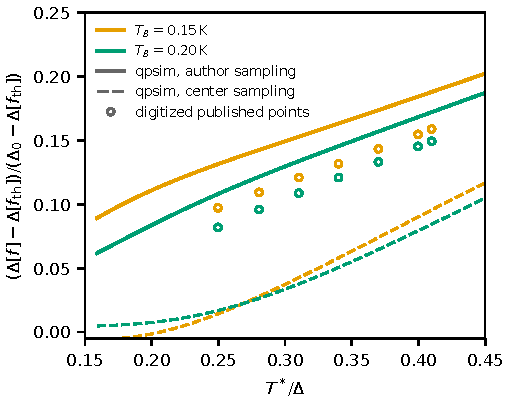
\includegraphics[width=\columnwidth]{fig_q0_curves.pdf}
\caption{\label{fig:q0}The author-semantics \qpsim{} endpoint over the
published window ($\mathrm{d}E = 1\ueV$, certificate-mode solves;
$T_B=0.15$~K at a documented one-decade-relaxed certificate at its
float64 floor).  Solid: the solved occupation read under the authors'
left-edge convention; dashed: the same states read at cell centers;
dash-dotted: the authors' own program, replayed in full (300/300
points converging under their Newton policy); open circles: the
published numerical curves digitized from the arXiv raster.  The
replayed author curves pass through the digitized points within
$0.12\times$ the digitization uncertainty, and lie \emph{between} the
two readings of the \qpsim{} solution family; $T_B=0.10$~K \qpsim{}
curves are excluded per Sec.~\ref{sec:certificates}.  Artifacts:
\texttt{fig6-Q0-sweep-de1-v1.json} (+\texttt{-t015-v1}),
\texttt{author-replay-sweep.json}.}
\end{figure}

\begin{figure}[t]
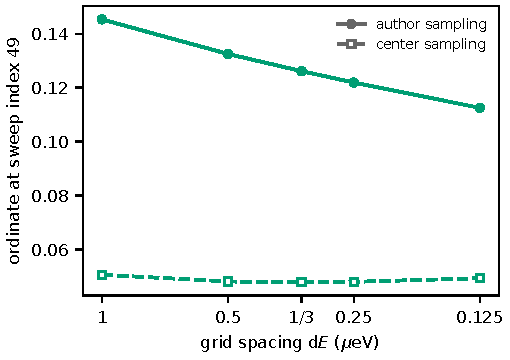
\includegraphics[width=\columnwidth]{fig_refinement.pdf}
\caption{\label{fig:refinement}Grid refinement of the anchored-point
ordinate ($T_B = 0.20$~K, sweep index 49) under both readings of the
re-solved root.  The center-carrier reading is grid-converged at the
published resolution; the left-edge reading is not.}
\end{figure}

Grid refinement at the anchored point ($T_B=0.20$~K, sweep index 49)
gives, for the re-solved root read under each convention:

\begin{table}[h]
\begin{ruledtabular}
\begin{tabular}{lccccc}
$\mathrm{d}E$ ($\ueV$) & 1 & 0.5 & 1/3 & 0.25 & 0.125 \\
\colrule
author sampling & 0.1454 & 0.1326 & 0.1262 & 0.1220 & 0.1125 \\
center sampling & 0.0505 & 0.0480 & 0.0477 & 0.0479 & 0.0492 \\
\end{tabular}
\end{ruledtabular}
\end{table}

\noindent
The two readings behave very differently but \emph{neither} is
continuum-converged at any resolution probed.  The center-carrier
reading varies only within $\pm 3\%$ across the full eightfold
refinement (with a shallow minimum near $\mathrm{d}E = 1/3\ueV$ and a
mild upturn at $0.125\ueV$), while the left-edge reading falls
monotonically by $23\%$ over the same range with sub-linearly decaying
differences.  The gap between the readings --- which must vanish as
$\mathrm{d}E \to 0$, since both discretize the same continuum
functional --- has closed by only about one third across the eightfold
refinement, decaying more slowly than $\sqrt{\mathrm{d}E}$.  Two
conclusions follow.  First, the published observable at the published
$1\ueV$ resolution, under its own sampling convention, carries a
discretization offset of at least $\sim 23\%$ relative to its own
$\mathrm{d}E = 0.125\ueV$ value --- comparable to the entire
inter-code discrepancy that motivated this study --- while the
center reading is the far more stable (though not strictly converged)
choice at practical resolutions.  Second, no single-resolution value of
this observable should be treated as converged: the solver residual
certifies to $10^{-12}$-level balance at every resolution shown while
the plotted number is still drifting, an instructive separation of
``solved'' from ``resolved.''  We deliberately refrain from a
continuum extrapolation --- the anomalously slow decay (consistent
with an edge-singularity-dominated error possibly compounded by the
resolution dependence of the near-threshold pair-breaking physics)
merits its own analytic treatment of the singular gap-edge cells.
\todo{physicist review of this paragraph before submission.}

\todo{Insert refinement figure (\texttt{fig\_refinement.pdf}) and the
$0.10/0.15$~K refinement columns; data:
\texttt{fig6-Q0-sweep-de2-v1.json}, \texttt{fig6-Q0-sweep-de4-v1.json},
\texttt{fig6-Q0-sweep-de2-t010-v1.json}.}

\section{Discussion and recommendations}

The campaign closes a two-code discrepancy without finding a physics bug
in either code, which is precisely why we think it is worth reporting.
Had we tuned kernels until the curves overlapped, we would have
``fixed'' correct physics.  The actionable conclusions:

\begin{enumerate}
\item \textbf{Report the sampling convention.}  For kinetic benchmarks
built from exponentially falling distributions under singular spectral
weights, state where on the grid the distribution is sampled and how the
observable quadrature pairs with that choice.  A half-bin ambiguity is
invisible in a methods section and worth a factor of two in a figure of
this construction.
\item \textbf{Demonstrate grid convergence of the plotted observable},
not merely of the solver residual.  The residual converges long before
the convention dependence of a ratio-of-small-differences observable is
resolved.
\item \textbf{Ratio observables amplify.}  The normalization
$\Delta_0 - \Delta[f_{\mathrm{th}}]$ is itself small; offsets that
perturb driven and thermal integrals unequally are magnified by an
order of magnitude or more in the plotted quantity.
\item \textbf{Near-threshold quadrature of pair-breaking deserves
analytic treatment.}  The per-bin error of the plain sum (up to $27\%$
in the closest bins here) is silent in aggregate observables but is a
real rate distortion at threshold.
\item \textbf{Component-substitution validation is practical.}  The
entire ladder --- authentication, clean-room port, seven substitutions,
independent verifiers, and machine-checked provenance --- was executed
against a single anchored point first, which is what made each
difference attributable.  Curve-level comparisons alone could not have
produced Table~\ref{tab:ladder}.
\end{enumerate}

\section*{Reproducibility}

Every completed stage is bound by a committed score and receipt carrying
SHA-256 digests of the immutable raw-array bundles, the complete source
closure (the full \qpsim{} tree plus all validation modules), and the
runtime; the independent verifiers use fixed-order compensated
summation with predeclared error bounds so their acceptance is
host-independent.  The authors' program is authenticated as
author-supplied reproduction source \todo{confirm redistribution /
citation terms with F\&C before publication}.  \todo{repository DOI /
release tag}.

\begin{acknowledgments}
We thank M.~Fischer and G.~Catelani for providing the program used to
produce the original figure. \todo{confirm; funding; colleagues.}
\end{acknowledgments}

\begin{thebibliography}{9}
\bibitem{fischer2023} M.~Fischer and G.~Catelani,
\todo{full citation of the 2023 Phys.\ Rev.\ Applied paper (Fig.~6)}.
\bibitem{kaplan1976} S.~B.~Kaplan, C.~C.~Chi, D.~N.~Langenberg,
J.~J.~Chang, S.~Jafarey, and D.~J.~Scalapino, Phys.\ Rev.\ B
\textbf{14}, 4854 (1976).
\todo{qpsim software citation; digitization/raster-oracle method note.}
\end{thebibliography}

\end{document}
